\subsection{实验环境}
\paragraph{系统} Ubuntu 16.04.3 LTS
\paragraph{CPU} Intel Core5

\subsection{实验结果}
\paragraph{计算逻辑准确性测试}
图\ref{fig:sys.param}展示了测试计算逻辑模块的准确性时,系统输出的结果。
\begin{figure}[H]
\begin{center}
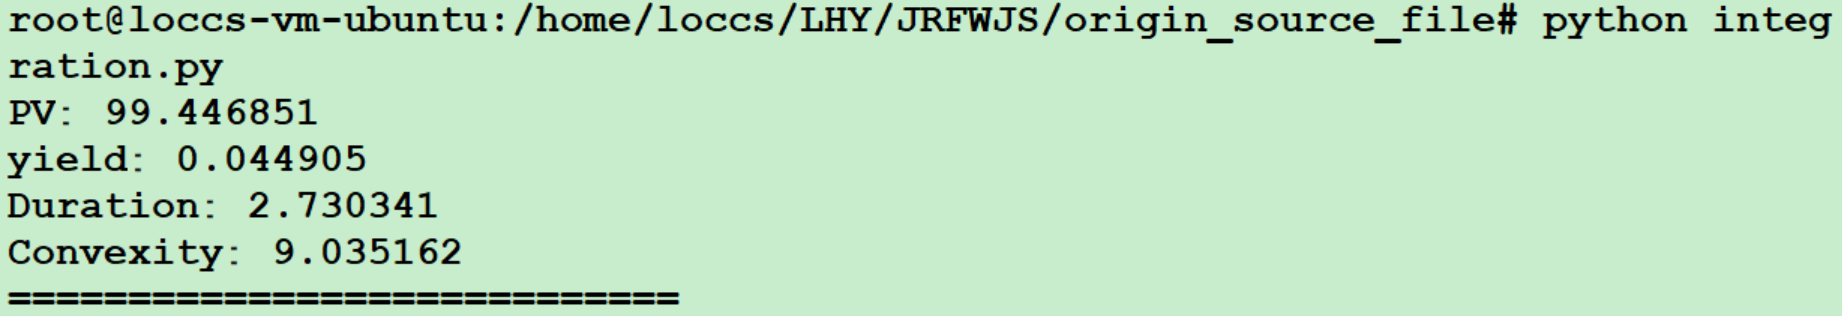
\includegraphics[width=16cm]{img//integration.PNG}
\caption{计算逻辑准确性测试}
\label{fig:sys.param}
\end{center}
\end{figure}


\paragraph{调用多进程性能测试}
图\ref{fig:sys.param}展示了调用Python多进程时,系统输出的结果。
\begin{figure}[H]
\begin{center}
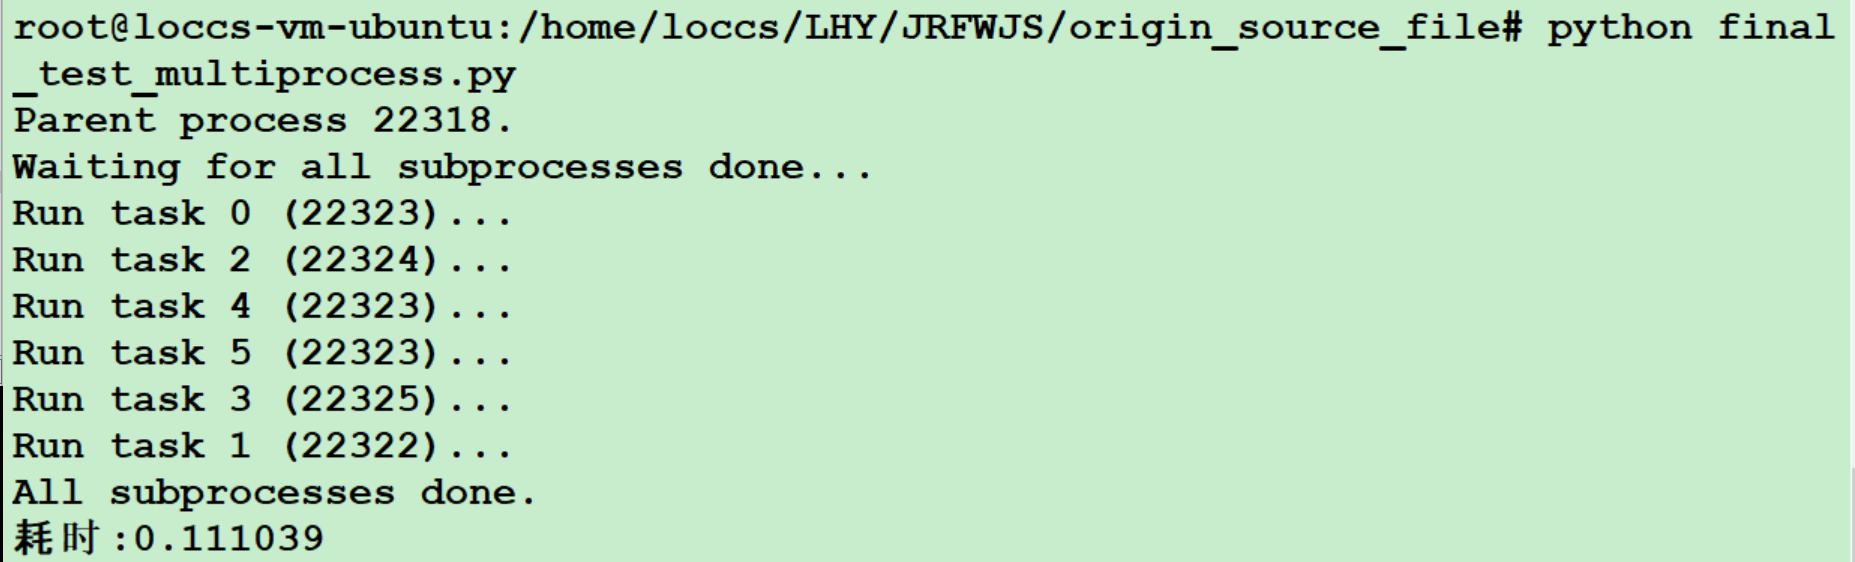
\includegraphics[width=16cm]{img//final_test_multiprocess.PNG}
\caption{调用多进程性能测试}
\label{fig:sys.param}
\end{center}
\end{figure}


\paragraph{自动测试结果}
图\ref{fig:sys.param}展示了使用自动测试程序测试本系统的准确性和性能时,自动测试程序输出的结果。
\begin{figure}[H]
\begin{center}
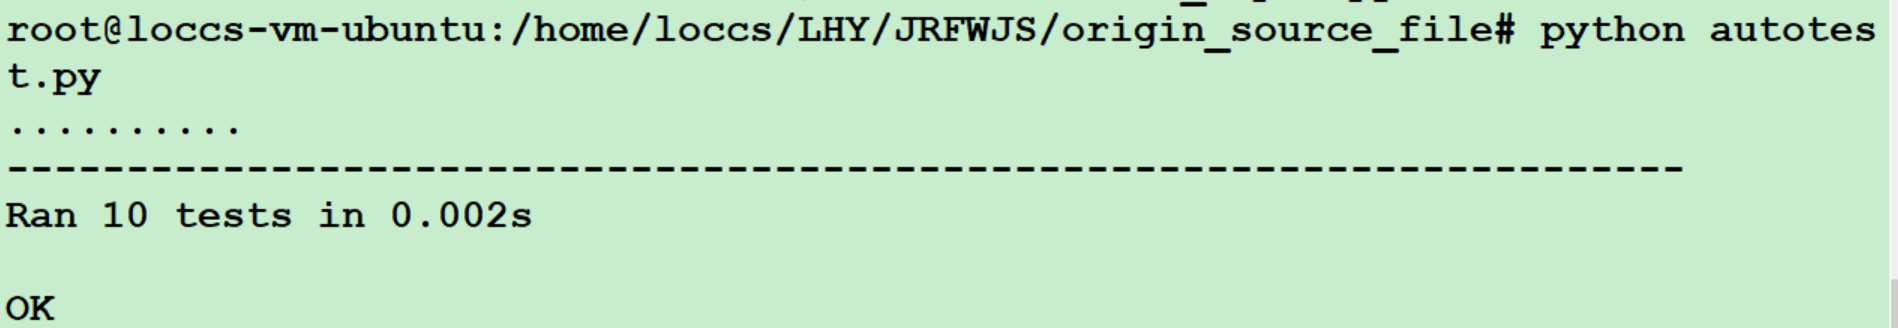
\includegraphics[width=16cm]{img//autotest.PNG}
\caption{自动测试结果}
\label{fig:sys.param}
\end{center}
\end{figure}


\paragraph{性能分析}在百万数据集上,调用C++加速。
\begin{table}[H]
\begin{adjustwidth}{-3cm}{-3cm}
\begin{center}
\begin{tabular}{|p{.8\textwidth}| p{.2\textwidth}|} \hline
技术手段 & 运行时间  \\ \hline
原始python代码 & 约50s  \\ \hline
使用Cython编译各函数 & 约38s  \\ \hline
使用Cython编译各函数并使用静态变量 & 约26s \\ \hline
\end{tabular}
\end{center}
\end{adjustwidth}
\end{table}

\paragraph{性能分析}在百万数据集上,调用Python多进程。
\begin{table}[H]
\begin{adjustwidth}{-3cm}{-3cm}
\begin{center}
\begin{tabular}{|p{.6\textwidth}| p{.2\textwidth}|p{.2\textwidth}|} \hline
技术手段 & 单进程时间 & 多进程时间 \\ \hline
原始python代码 & 约50s  & 约13s\\ \hline
使用Cython编译各函数 & 约38s  & 约11s\\ \hline
使用Cython编译各函数并使用静态变量 & 约26s & 约7.8s\\ \hline
\end{tabular}
\end{center}
\end{adjustwidth}
\end{table}
